\section{PDCA}\label{app:pdca}
I processi sono organizzati in modo da permetterne un miglioramento continuo.\\
Per attuare tale miglioria è necessario che i processi seguano un ciclo che ne determini l'evoluzione nel tempo.
A questo scopo verrà utilizzato il Ciclo di Deming qui definito.
\begin{itemize}
	\item \textbf{Plan} - \textit{Pianificazione}: definire attività, scadenze, responsabilità.
	\item \textbf{Do} - \textit{Esecuzione} : esecuzione della pianificazione.
	\item \textbf{Check} - \textit{Valutazione}: valutazione dei risultati ottenuti e confronto con le previsioni della pianificazione. 
	\item \textbf{Act} - \textit{Azione}: correzione delle criticità, presa d’atto di risultati positivi con relativa standardizzazione dei processi corretti.
\end{itemize}
%\begin{figure}
%	\centering
%	\begin{subfigure}
%	\centering
%	\includesvg[width=5cm]{PDCA}
%	\caption{Ciclo PDCA}
%	\end{subfigure}%
%	\begin{subfigure}
%		\centering
%		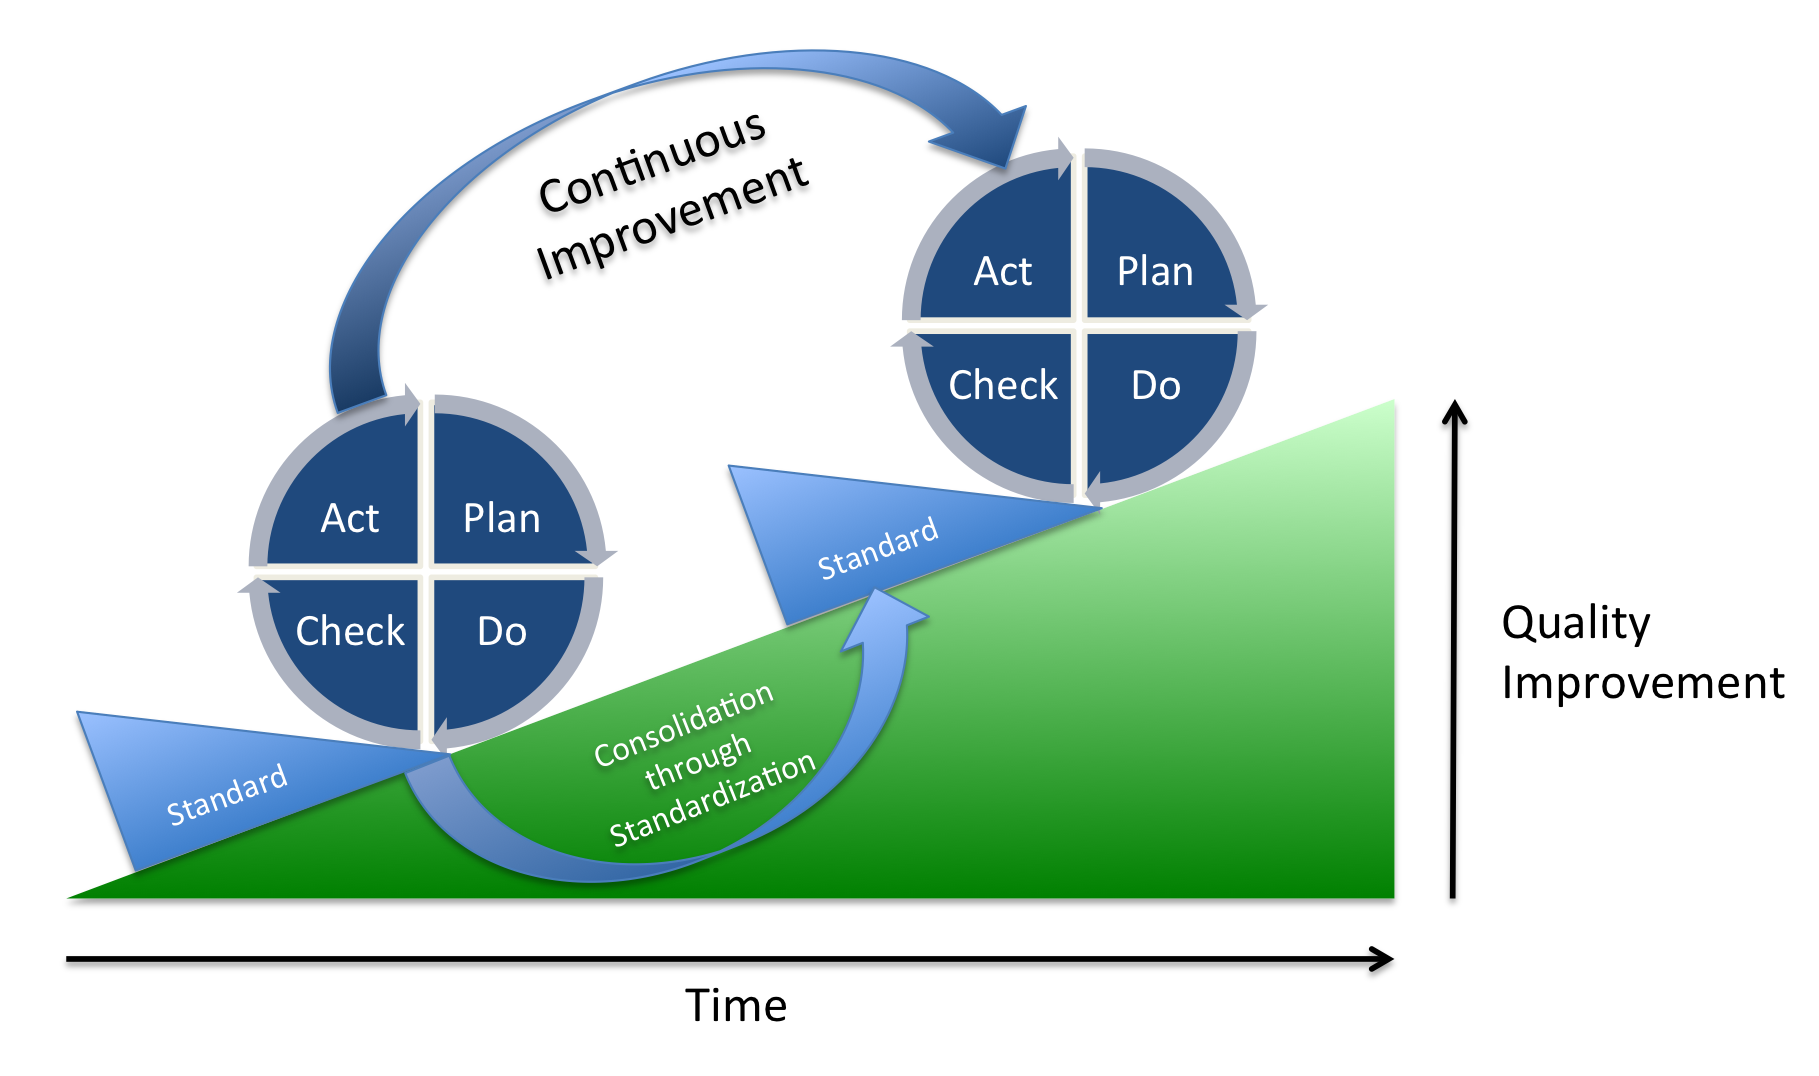
\includegraphics[width=10cm]{PDCAProcess}
%		\caption{Miglioramento continuo della qualità con PDCA}
%	\end{subfigure}
%\end{figure}
\begin{figure}[H]	
	\centering
	\includesvg[width=8cm]{PDCA}
	\caption{Ciclo PDCA}
\end{figure}
\begin{figure}[H]
	\centering
	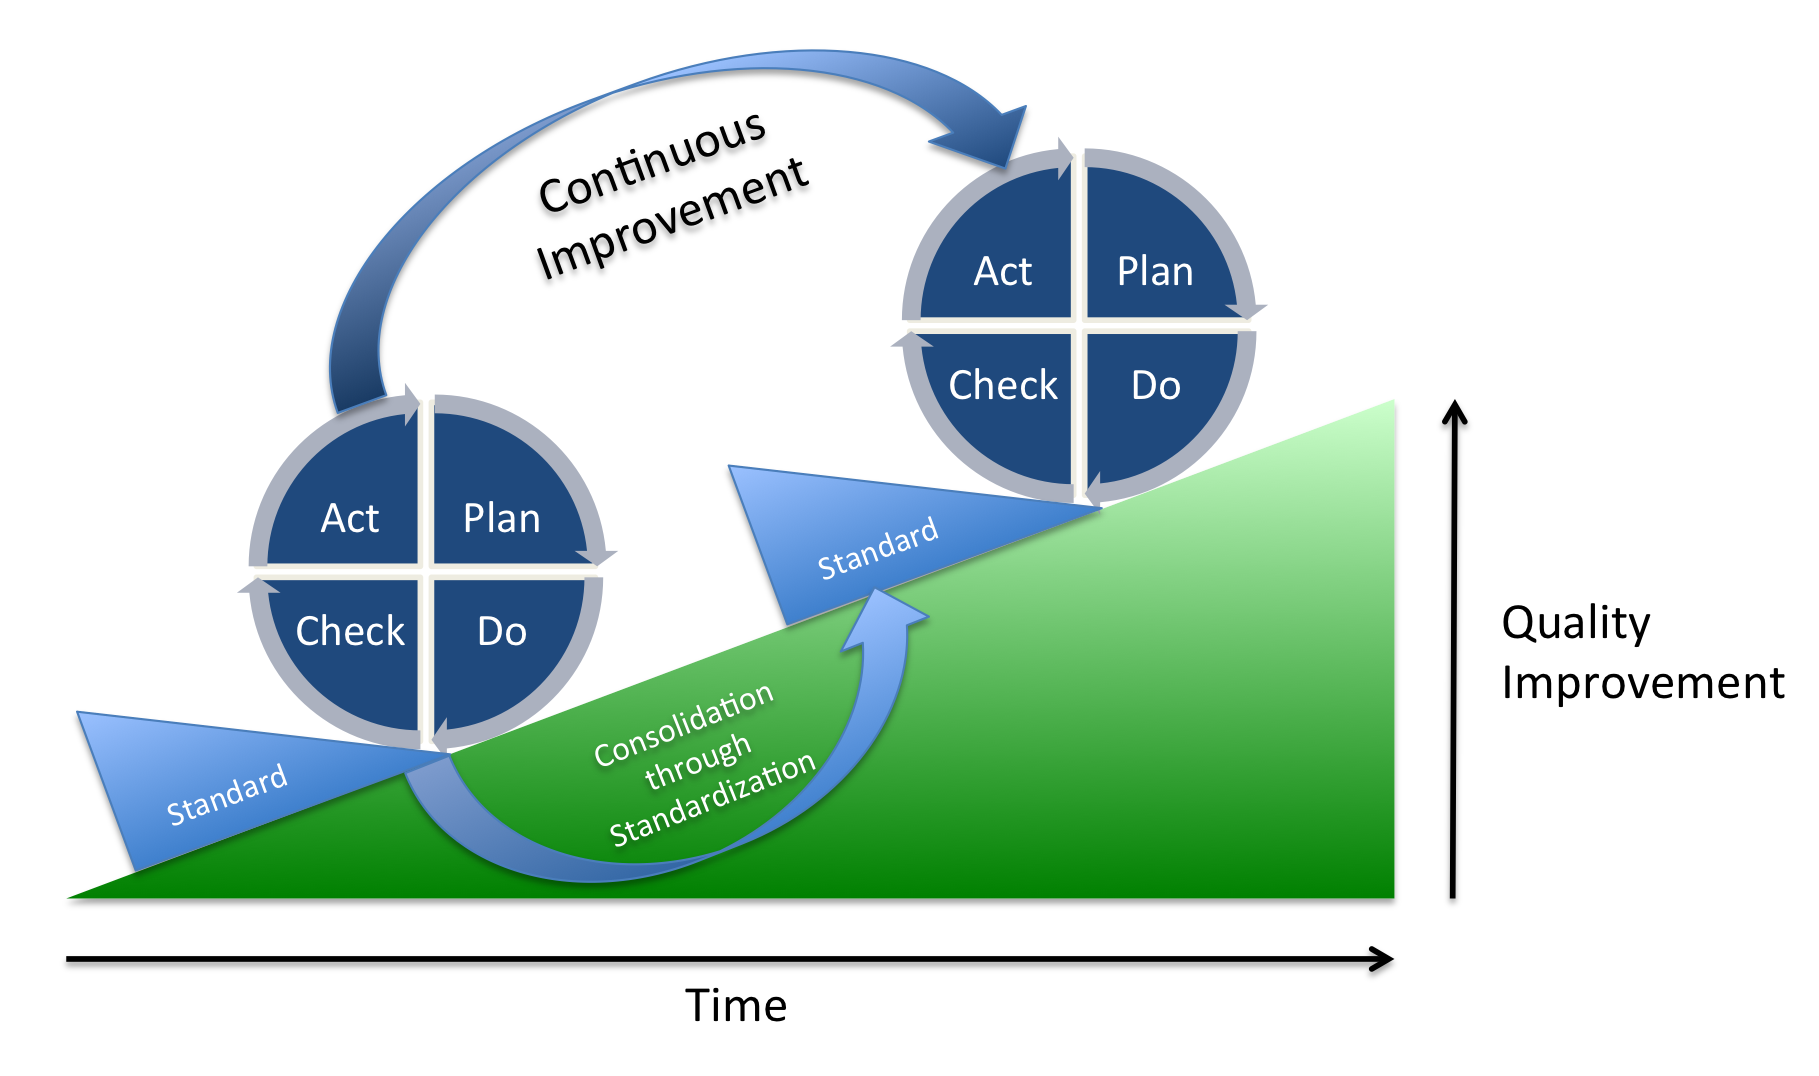
\includegraphics[width=10cm]{PDCAProcess}
	\caption{Miglioramento continuo della qualità con PDCA}
\end{figure}